\documentclass[12pt]{article}

\usepackage{listings}
\usepackage{graphicx}
\usepackage{float}
\usepackage{hyperref}
\usepackage{ifthen}

\usepackage{amssymb} 
\usepackage{amsmath}
\usepackage{amsthm}
\usepackage{sansmath}
\usepackage{epsfig}

\usepackage[T1]{fontenc}
\usepackage{lmodern}
\renewcommand*\familydefault{\sfdefault}

\usepackage[margin=2cm]{geometry}

\usepackage[parfill]{parskip}
\linespread{1.2} 

\usepackage{xcolor}

\lstdefinestyle{code}{  
    commentstyle=\color{gray},
    keywordstyle=\color{blue},
    numberstyle=\tiny\color{gray},
    stringstyle=\color{teal},
    ndkeywordstyle=\color{purple},
    basicstyle=\ttfamily\footnotesize,
    breakatwhitespace=false,         
    breaklines=true,                 
    captionpos=t,                    
    keepspaces=true,                 
    numbers=left,                    
    numbersep=8pt,                  
    showspaces=false,                
    showstringspaces=false,
    showtabs=false,                  
    tabsize=4,
    frame=single,
    breaklines=true
}

\lstset{style=code}

\newcounter{question}
\setcounter{question}{4}
\newcounter{subquest}

\newcommand{\question}[1]{
    \stepcounter{question} 
    \ifnum\value{question}>1 \fi
    \vspace{.5em}
    \textbf{ \Large\thequestion \ - #1} \\
    \vspace{.5em} 
    \hrulefill \\
    \setcounter{subquest}{0}\ }

\newcommand{\subquestion}[1][true]{
    \stepcounter{subquest} 
    \ifthenelse{\equal{#1}{true} \and \value{subquest}>1}{\newpage}{}
    \vspace{1em}
    \textbf{\large Question \thequestion.\thesubquest}
    \vspace{.5em}\ \\}

\newcommand{\solution}
    {\hrulefill \par\vspace{0.5em}\noindent\emph{Solution.}\ }
    {\par\vspace{1em}}

\newcommand{\startappendix}{%
    \newpage
    \vspace{1em}
    {\Large\textbf{Appendix}}

    The complete code used for this assignment is provided in the appendix for reference. Files can be accessed directly at this \href{https://github.com/sjsusu/numerical_analysis}{GitHub repository}.
}

\usepackage{fancyhdr}
\setlength{\headheight}{15pt}
\pagestyle{fancy} 
\lhead{Math 5335: \emph{Numerical Analysis}}
\rhead{Homework 5}
\cfoot{}
\rfoot{\thepage}

\begin{document}
\setcounter{page}{6}
\question{FEM Implementation}
For the python implmentation, we used:
\begin{itemize}
    \item The global and elemental indexing schemes for the nodes and elements.
    \item The previously derived formulas of the coefficients for the basis functions $\phi_i$, elementary stiffness elements $A^{k}_{ij}$, and elementary load elements $F^{k}_i$.
    \item Initial and Boundary condition implementation by:
    \begin{itemize}
        \item Zeroing out the rows and columns of the stiffness matrix corresponding to the boundary nodes.
        \item Setting the diagonal entries of the stiffness matrix for the boundary nodes to 1.
        \item Setting the corresponding entries in the load vector to the boundary condition values.
    \end{itemize}
    \item After assembly, we used Scipy's linear solver to generate the solution vector.
\end{itemize}

The general structure of the code is as follows:
\begin{enumerate}
    \item Define mesh dimensions and parameters.
    \item Generate a global node index, element connectivity, and elemental nodal value matrices.
    \item Generate elemental stiffness matrices and load vectors, and assemble them into the global stiffness matrix and load vector.
    \item Enforce initial and boundary conditions by modifying the stiffness matrix and load vector.
    \item Solve the resulting linear system to obtain the solution at the nodes.
    \item Plotting and error computation.
\end{enumerate}

\newpage 
\lstinputlisting[language=Python, caption={FEM Python Implementation}]{../hw5.py}

\newpage
\question{Results and Bonus Questions}
Given $N=6$ and $M=4$, we obtained the following plots:
\begin{center}
    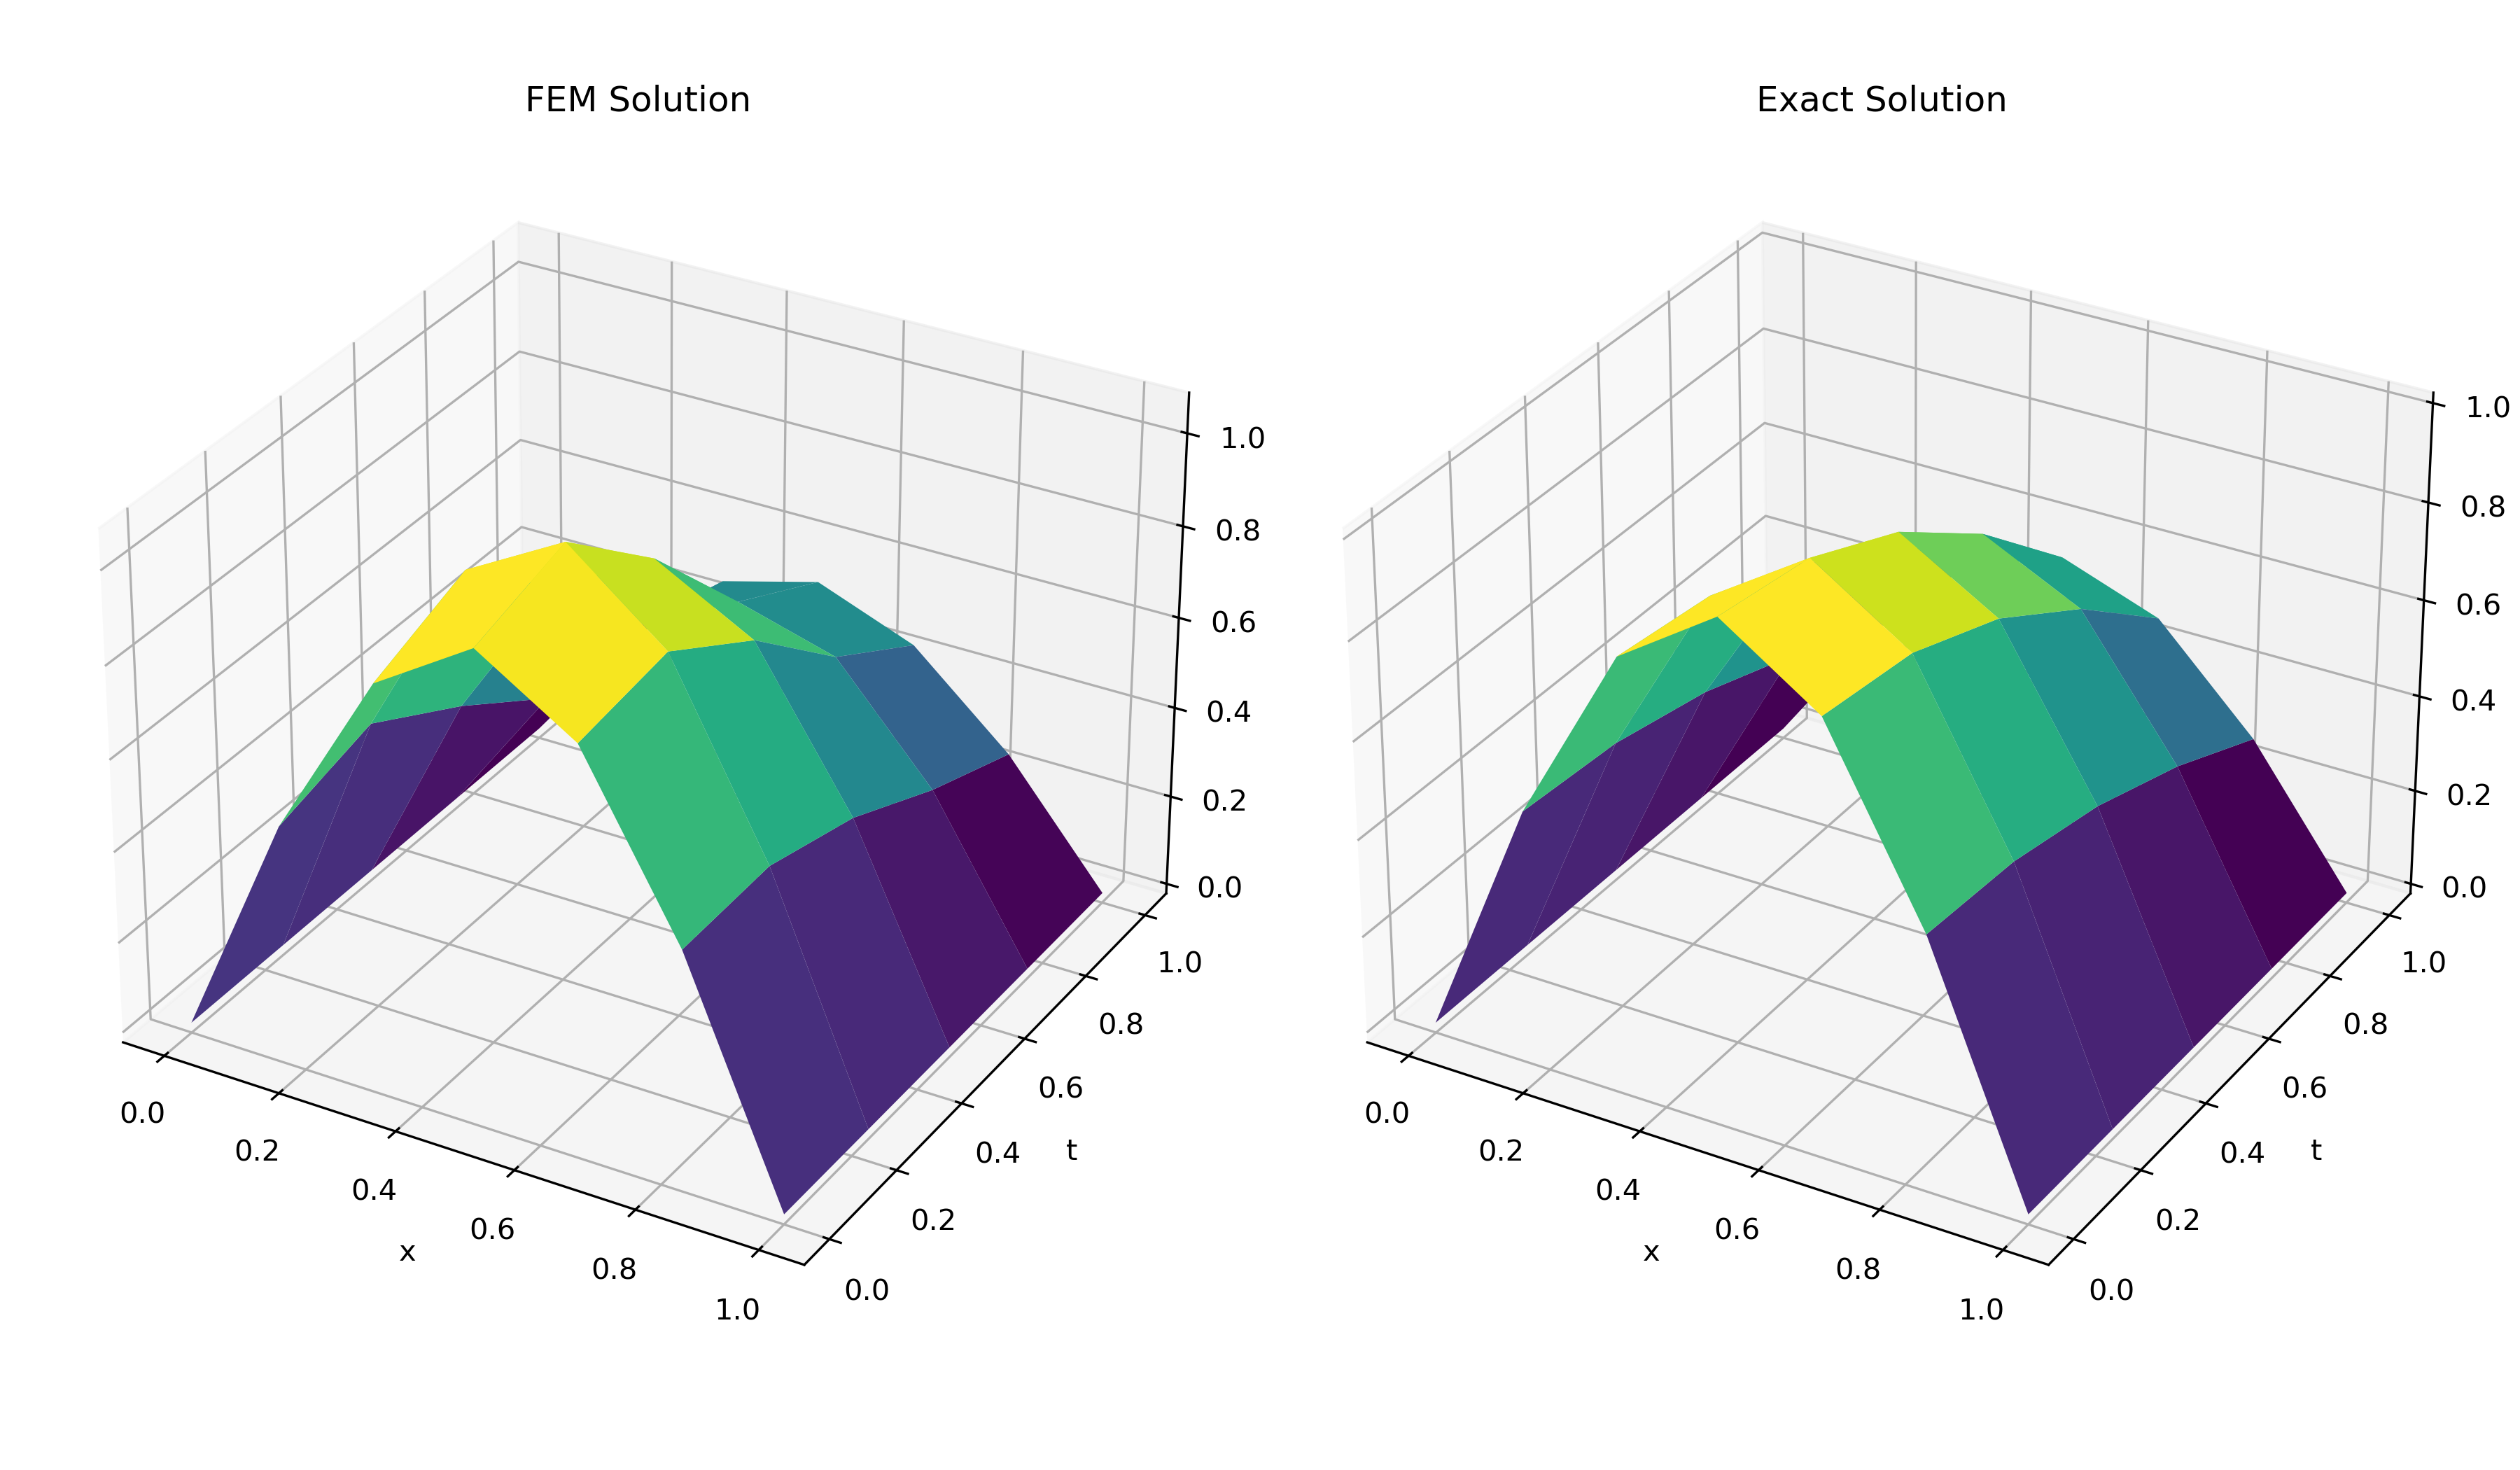
\includegraphics[width=0.9\textwidth]{../N6_M4.png}
\end{center}
The maximum nodal error was approximately $0.11107680006432841$.

Increasing the mesh resolution to $N=12$ and $M=8$, we obtained the following plots:
\begin{center}
    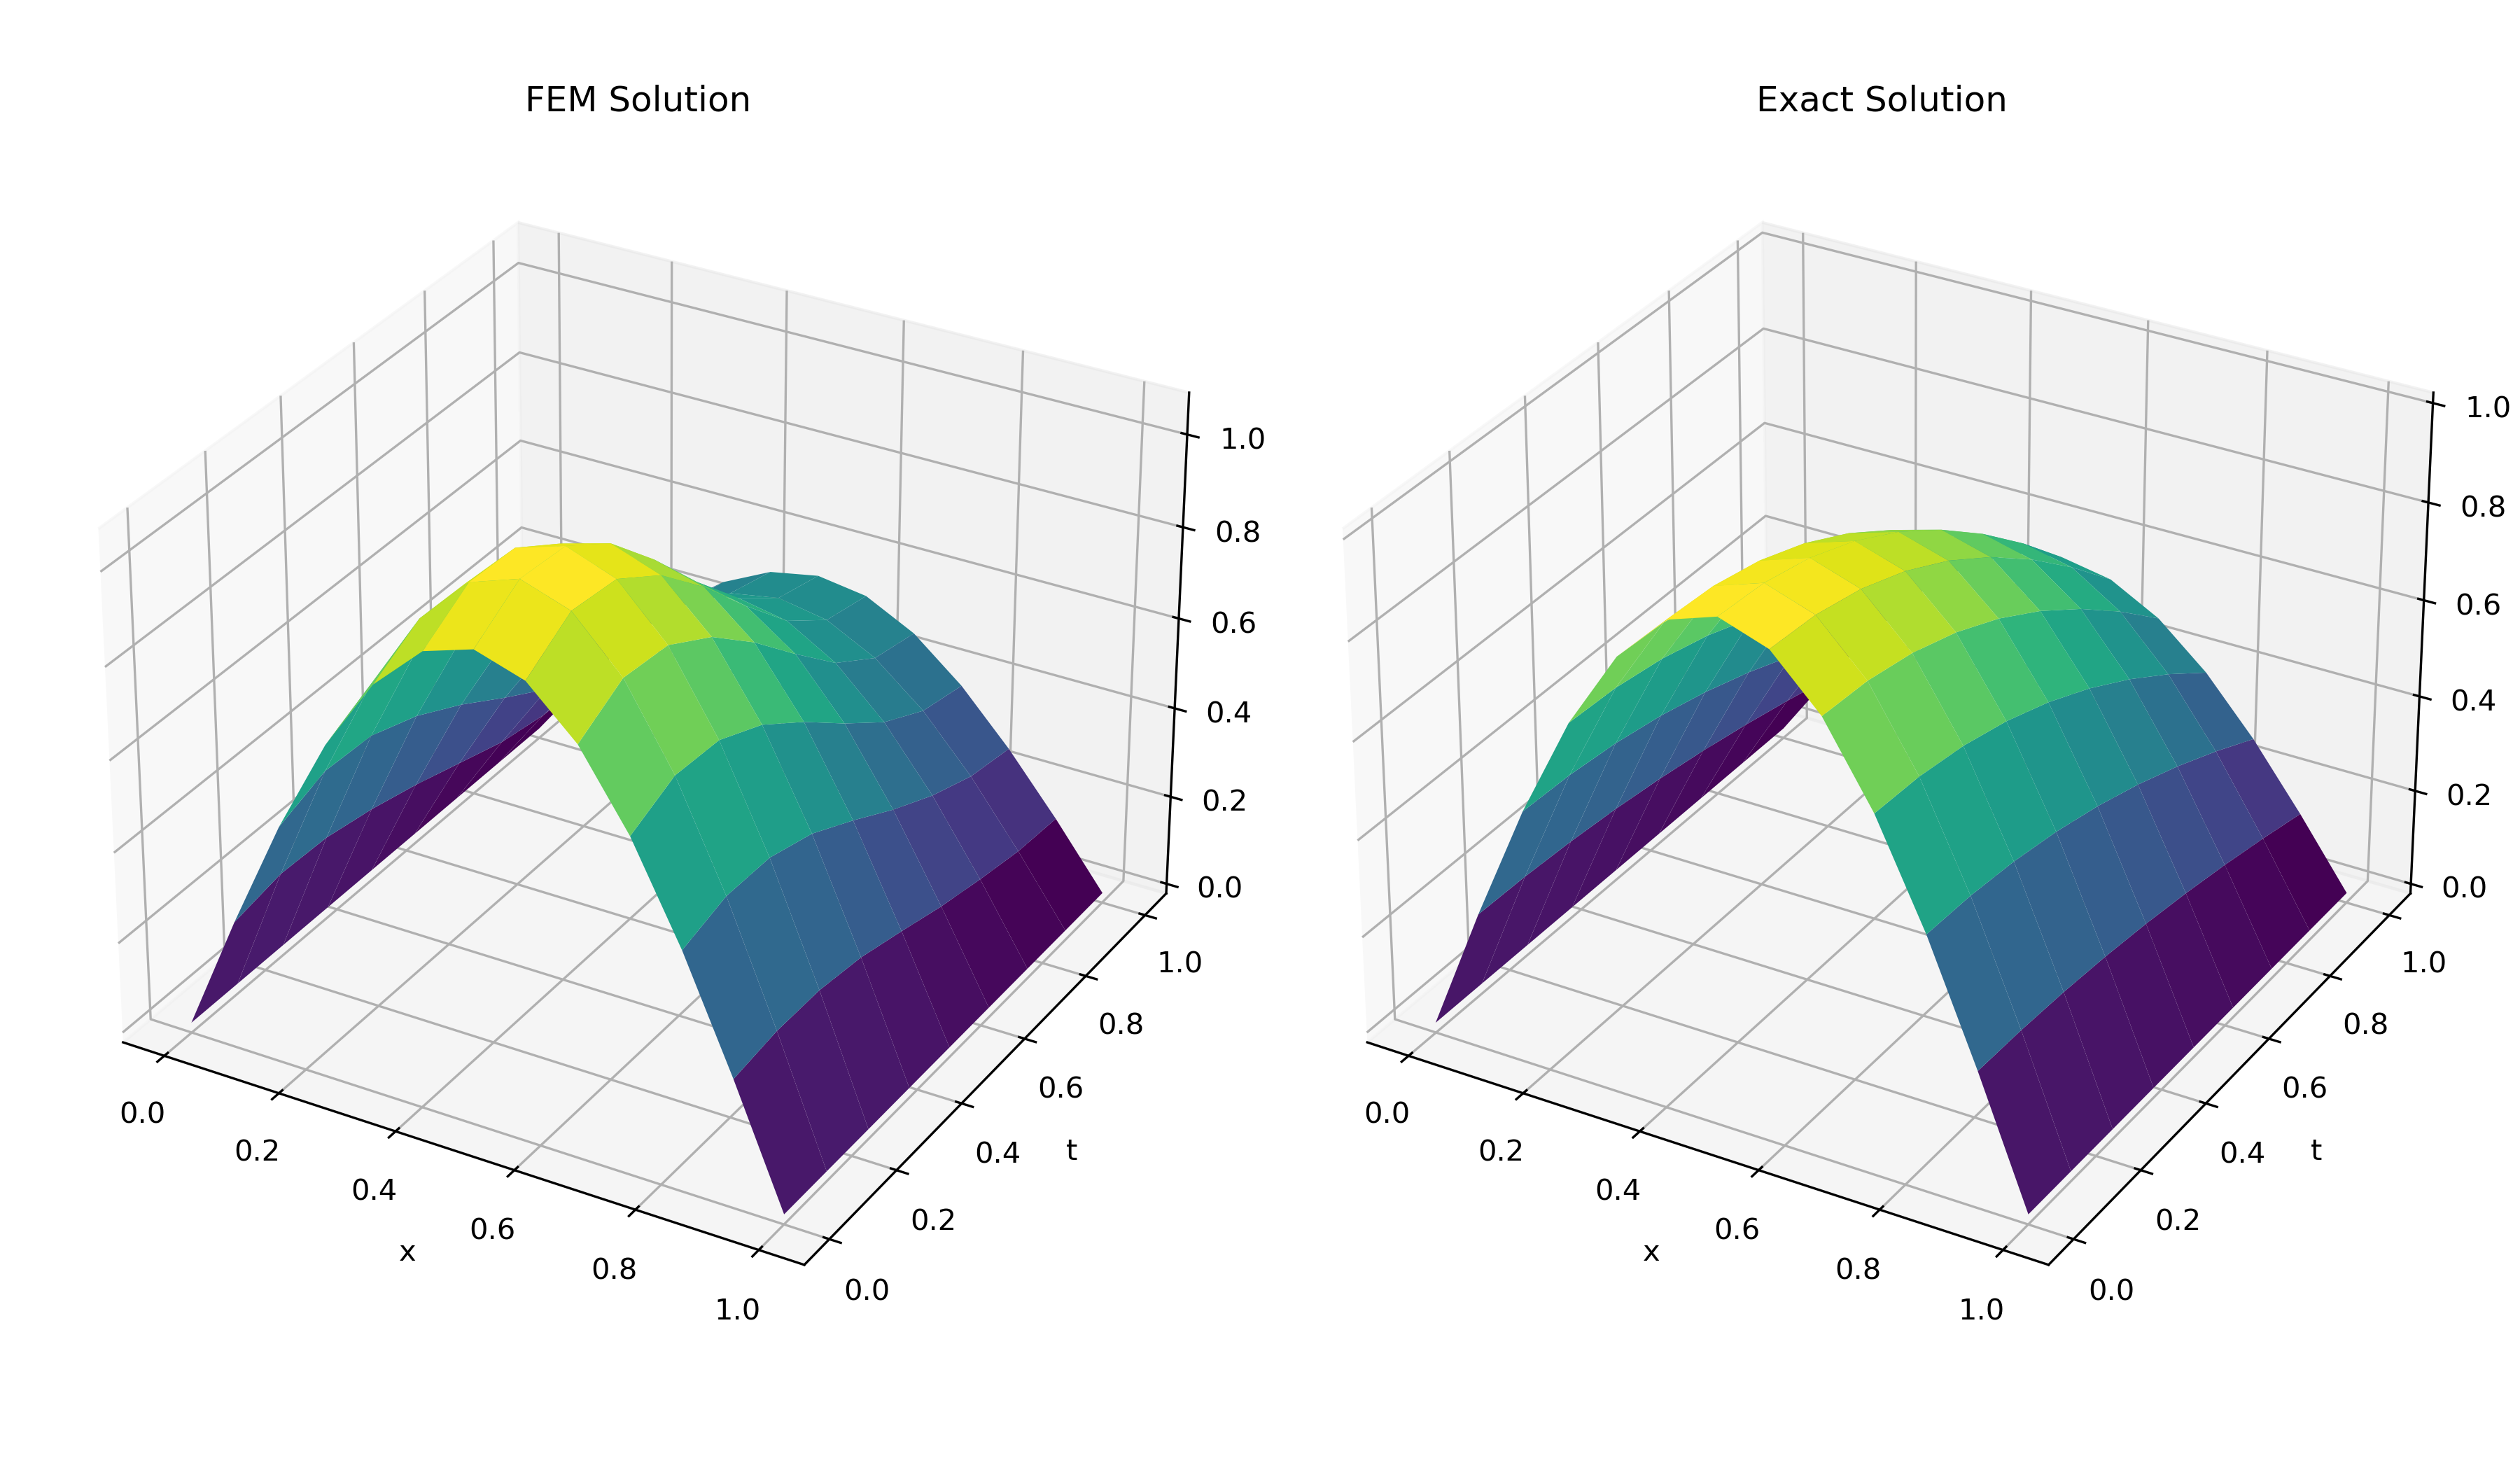
\includegraphics[width=0.9\textwidth]{../N12_M8.png}
\end{center}
The maximum nodal error was approximately $0.0911792636573886$.

We observe that our numerical solution captures the general behavior of the exact solution. However, there are some notable discrepancies around $t=0.8$, where the approximation appears to be dampened compared to the exact solution. This could be due to the choice of a single point quadrature rule, which may not be sufficient to capture the curvature/oscillation completely. An increase in the number of quadrature points or a higher-order quadrature method could potentially improve the accuracy in this region.

In refining the mesh, we observed a reduction in the maximum nodal error. An additional refinement of the mesh to $N=24$ and $M=16$ showed another decrease in error. This is consistent with the expectation that a finer mesh should yield a more accurate approximation to the exact solution.

\end{document}